\documentclass{beamer}
\usepackage{listings}
\lstset{
%language=C,
frame=single, 
breaklines=true,
columns=fullflexible
}
\usepackage{blkarray}
\usepackage{subcaption}
\usepackage{url}
\usepackage{tikz}
\usepackage{tkz-euclide} % loads  TikZ and tkz-base
%\usetkzobj{all}
\usetikzlibrary{calc,math}
\usepackage{float}
\newcommand\norm[1]{\left\lVert#1\right\rVert}
\renewcommand{\vec}[1]{\mathbf{#1}}
\newcommand{\myvec}[1]{\ensuremath{\begin{pmatrix}#1\end{pmatrix}}}
\usepackage[export]{adjustbox}
\usepackage[utf8]{inputenc}
\usepackage{amsmath}
\usepackage{tikz}
\DeclareFontShape{OT1}{cmss}{b}{n}{<->ssub * cmss/bx/n}{}
\usetikzlibrary{automata, positioning}
\usetheme{Boadilla}
\providecommand{\sbrak}[1]{\ensuremath{{}\left[#1\right]}}
\providecommand{\lsbrak}[1]{\ensuremath{{}\left[#1\right.}}
\providecommand{\rsbrak}[1]{\ensuremath{{}\left.#1\right]}}
\providecommand{\pr}[1]{\ensuremath{\Pr\left(#1\right)}}
\providecommand{\brak}[1]{\ensuremath{\left(#1\right)}}
\providecommand{\lbrak}[1]{\ensuremath{\left(#1\right.}}
\providecommand{\rbrak}[1]{\ensuremath{\left.#1\right)}}
\providecommand{\cbrak}[1]{\ensuremath{\left\{#1\right\}}}
\providecommand{\lcbrak}[1]{\ensuremath{\left\{#1\right.}}
\providecommand{\rcbrak}[1]{\ensuremath{\left.#1\right\}}}
\let\vec\mathbf
\newcommand*{\permcomb}[4][0mu]{{{}^{#3}\mkern#1#2_{#4}}}
\newcommand*{\perm}[1][-3mu]{\permcomb[#1]{P}}
\newcommand*{\comb}[1][-1mu]{\permcomb[#1]{C}}

\title{GATE EE EXAM (2012), Question 47}
\author{Amaan}
\date{June 21,2021} 
\begin{document}

\begin{frame}
\titlepage
\end{frame}

\begin{frame}
    \frametitle{Prerequisites}
    \begin{block}{State Space}
      The set of all possible states the system/object can be in. Without loss in generality, the state space can be identified with the set $S=\{ 1,2,\dots,\ell\}$, where $\ell$ is a fixed arbitrary natural number.
    \end{block}
    \begin{block}{Random Variables}
     Let $\{ X_0,X_1,X_2\dots\}$ be a sequence of discrete random variables, where each $X_t \in S$, and $X_t$ represents the state of the system at time $t$.
    \end{block}
\end{frame}

\begin{frame}
    \frametitle{Prerequisites Contd.}
    \begin{block}{Markov Processes and Markov Chains}
     \begin{itemize}
    \item A process is said to be a Markov Process if the probability of transitioning to any particular state is dependent solely on the current state and does not depend on how the current state was reached.
    \item Mathematically, $ \{X_0,X_1,\ldots\}$ is called a  Markov chain if 
 \begin{align}
    \pr{(X_{n}=i_n\mid X_{n-1}=i_{n-1},\ldots,X_0=i_{0}}= \pr{X_{n}=i_n\mid X_{n-1}=i_{n-1}}
    \label{eq1}
 \end{align}
     \end{itemize}
\end{block}
\end{frame}

\begin{frame}
\frametitle{Prerequisites Contd.}
    \begin{block}{Transition Matrix}
     \begin{itemize}
        \item  For each pair $ i,j\in S$, consider the (conditional) probability $ p_{ij}\in[0,1]$ for the transition of the object or system from state $ i$ to $ j$ within one time step.
        \item The $ \ell\times\ell$ matrix $ {\mathbf{P}}=(p_{ij})_{i,j=1,\ldots,\ell}$ of the transition probabilities $ p_{ij}$ where
        \begin{align}
            p_{ij}\ge0\,,\qquad p_{ij}=\pr{X_{n+1}=j\mid X_{n}=i}	
            \label{eq2}
        \end{align}
        is called one-step \textit{transition matrix} or simply transition matrix of the Markov chain.
    \end{itemize}
    \end{block}
\end{frame}

\begin{frame}
    \frametitle{Prerequisites Contd.}
     \begin{block}{Definition 1}
         The standard form of a state transition matrix is,
         \begin{align}
   \vec{P}=\begin{blockarray}{ccc}
&A & N \\
\begin{block}{c[cc]}
  A & \vec{I} & \vec{O}  \\
  N & \vec{R} & \vec{Q} \\
\end{block}
\end{blockarray}
\label{eq3}
\end{align}
where,
    $A$ and $N$ are Absorbing and Non-absorbing states.$\vec{I}$ is the Identity matrix, $\vec{O}$ being the Null matrix, and $\vec{R},\vec{Q}$ are other sub-matrices.\\
\end{block}
\end{frame}
\begin{frame}
    \frametitle{Prerequisites Contd.}
    \begin{block}{Definition 2}
      The limiting matrix for absorbing Markov chain is,
\begin{align}
    \vec{\bar P}= \lim_{n\to\infty} \vec P^{n} =\begin{bmatrix}
    \vec{I} & \vec{O}\\
    \vec{FR} & \vec{O}\\
    \end{bmatrix}
    \label{eq4}
\end{align}
\\where,
\begin{align}
    \vec{F}=(\vec{I}-\vec{Q})^{-1}
    \label{eq5}
\end{align}
is called the fundamental matrix of $\vec{P}$. \\
    \end{block}
\end{frame}
\begin{frame}{Prerequisites Contd.}
\begin{block}{Definition 3}
A element $\bar p_{ij}$ of $\vec{\bar P}$ denotes the absorption probability in state $j$, starting from state $i$.
\end{block}
\end{frame}
\begin{frame}
    \frametitle{Question}
    \begin{block}{GATE EE EXAM (Dec 2012), Question 47}
   A fair coin is tossed till head appears for the first time. The probability that the number of required tosses is odd, is, \\
\begin{enumerate}
    \item $\frac{1}{3}$
    \item $\frac{1}{2}$
    \item $\frac{2}{3}$
    \item $\frac{3}{4}$
\end{enumerate}
  \end{block}
\end{frame}
\begin{frame}
\frametitle{Solution}
    Given, a fair coin is tossed till heads turns up,
\begin{align}
p=\dfrac{1}{2},q=\dfrac{1}{2}
\label{eq6}
\end{align}
    Let us define a Markov chain $\{X_{0},X_{1},X_{2}\dots\}$, where $X_{n}\in S$ \vee $n\in\{0,1,2,\dots\}$, and $S=\{1,2,3,4\}$ is the state space.
   \begin{table}[h!]
\centering
\caption{Definition of Random Variables}
\label{table:1}
\begin{tabular}{|c|c|c|}
    \hline
    R.V & Value=0 & Value=1 \\
    \hline
    $X$ & $N_{tosses}=2k$ & $N_{tosses}=2k-1$ \\[1ex]
    \hline
    $Y$ & $H$ & $T$ \\[1ex]
    \hline
\end{tabular}
\end{table}    
\end{frame}
\begin{frame}
 \frametitle{Solution Contd.}
 The definition of state space $S$,
      \begin{table}[h!]
\centering
\caption{Markov states and Notations }
\label{table:2}
\begin{tabular}{|c|c|}
    \hline
    Notation & State \\
    \hline
    $S=1$ & $(X,Y)=(0,1)$ \\[1ex]
    \hline
    $S=2$ & $(X,Y)=(1,1)$\\[1ex]
    \hline
    $S=3$ & $(X,Y)=(0,0)$\\[1ex]
    \hline
    $S=4$ & $(X,Y)=(1,0)$\\[1ex]
    \hline
\end{tabular}
\end{table}
\end{frame}
\begin{frame}
  \frametitle{Solution Contd.} 
  
   \begin{figure}[h]
\caption*{\textbf{Markov chain diagram}}
\centering
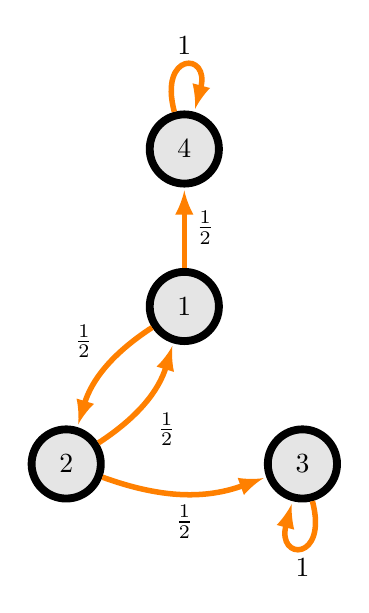
\begin{tikzpicture}
    % Setup the style for the states
        \tikzset{node style/.style={state, 
                                    minimum width=0.15cm,
                                    line width=1mm,
                                    fill=gray!20!white}}
        % Draw the states
        \node[node style] at (1.5, -2)      (bull) {1};     
        \node[node style] at (0, -4)      (bear) {2};      
        \node[node style] at (3, -4)     (over1) {3};  
        \node[node style] at (1.5, 0)      (over2) {4}; 
        % Connect the states with arrows
        \draw[every loop,
              auto=right,
              line width=0.7mm,
              >=latex,
              draw=orange,
              fill=orange]
        (bull) edge[bend right = 20] node{$\frac{1}{2}$} (bear)
        (bear) edge[bend right = 20] node{$\frac{1}{2}$}
        (bull)
        (bear) edge[bend right = 20] node{$\frac{1}{2}$}
        (over1)
        (over1) edge[loop below] node{1}
        (over1)
        (bull) edge node{$\frac{1}{2}$} (over2)
        (over2) edge[loop above] node{1} (over2) ;
\end{tikzpicture}
\end{figure}
\end{frame}

\begin{frame}
  \frametitle{Solution Contd.} 
  For the above discussed Markov Chain, the states 3 and 4 are the Absorbing states, and, 1 and 2 are Non-absorbing states, 
      \begin{block}{Corollary 1}
        The state transition matrix for the above Markov chain is, 
\begin{align}
    \vec{P}=\begin{blockarray}{cccccc}
& 3 & 4 & 1 & 2 \\
\begin{block}{c[ccccc]}
  3 & 1 & 0 & 0 & 0 \\
  4 & 0 & 1 & 0 & 0 \\
  1 & 0 & 0.5 & 0 & 0.5  \\
  2 & 0.5 & 0 & 0.5 & 0  \\
\end{block}
\end{blockarray}
\label{eq7}
\end{align} 
      \end{block}
\end{frame}

\begin{frame}
 \frametitle{Solution Contd.}
 From \eqref{eq3} and \eqref{eq7}, we get,
\begin{align}
    \vec{R}=\begin{bmatrix}
    0 & 0.5\\
    0.5 & 0\\
    \end{bmatrix},
    \vec{Q}=\begin{bmatrix}
    0 & 0.5 \\
    0.5 & 0 \\
    \end{bmatrix}
    \label{eq8}
\end{align}     
\begin{block}{Corollary 2}
  Limiting Matrix of the Markov chain under observation is, 
\begin{align} 
    \vec{\bar P}=\begin{blockarray}{ccccc}
&3 &4 &1 &2\\
\begin{block}{c[cccc]}
    3 & 1 & 0 & 0 & 0  \\
    4 & 0 & 1 & 0 & 0  \\
    1 & \frac{1}{3} & \frac{2}{3} & 0 & 0 \\
    2 & \frac{2}{3} & \frac{1}{3} & 0 & 0 \\
   \end{block}
\end{blockarray}
\label{eq9}
\end{align}
\end{block}
\end{frame}

\begin{frame}
  \frametitle{Solution Contd.} 
   \begin{block}{Corollary 3}
       The required probability is,
\begin{align}
P =\bar p_{14}
\label{eq10}
\end{align}
From \eqref{eq9} and \eqref{eq10},
\begin{align}
P=\frac{2}{3}
\end{align}
   \end{block}
$\therefore$ option 3 is correct.   
\end{frame}

\end{document}